\documentclass[presentation]{beamer}
\mode<presentation>{\usetheme{AMSBolognaFCrev}}

\usepackage[utf8]{inputenc}
\usepackage[T1]{fontenc}
\usepackage{booktabs}
\usepackage{array}
\usepackage{tabularx}
\usepackage{tikz}
\usepackage[ddmmyyyy]{datetime}
\usepackage[export]{adjustbox}
\usetikzlibrary{arrows.meta,positioning,shapes.geometric,fit,calc}

\renewcommand{\dateseparator}{/}
\newcommand{\sectiontitleframe}[1]{
\begin{frame}[plain,c]
\begin{center}
{\usebeamerfont{title}\usebeamercolor[fg]{title}#1}
\end{center}
\end{frame}
}

\tikzset{
    labbox/.style={draw, rounded corners, align=center, font=\scriptsize,
        minimum height=0.72cm, text width=2.05cm},
    smalllabbox/.style={draw, rounded corners, align=center, font=\tiny,
        minimum height=0.55cm, text width=1.65cm},
    labarrow/.style={-{Stealth[length=2mm]}, thick}
}

\title[Lesson 7]{OpenHospital API Network Security Lab}
\institute[Data Privacy and Security]{Healthcare Data Privacy and Security}
\author[\sspeaker{G. Pisano}]{\speaker{Giuseppe Pisano} \\\href{mailto:g.pisano@unibo.it}{g.pisano@unibo.it}}
\date[August, 2026]{August, 2026}
%
\titlegraphic{
\begin{center}
    
\includegraphics[width=0.35\textwidth, valign=c]{logos/intestazione.png}
    
\includegraphics[width=0.16\textwidth, valign=c]{logos/unibo_logo_2.png}
    
\includegraphics[width=0.11\textwidth, valign=c]{logos/makeni_logo_2.png}
    
\includegraphics[width=0.20\textwidth, valign=c]{logos/cuamm_logo_png.png}
\end{center}
\centering
\tiny{S.K.I.L.L.E.D --- AID013244/04/2\\Strategic Knowledge and Inclusive Lifelong Learning in the health sector for youth Employability and Development}
}

\newcommand{\scenario}{St. Isidore Hospital}
\newcommand{\takeawaysframe}[2]{
\begin{frame}[c]{Recap: \insertsection}
\begin{block}{Takeaways}
#1
\end{block}
\begin{exampleblock}{In \scenario}
#2
\end{exampleblock}
\end{frame}
}

\begin{document}

\setbeamertemplate{frametitle}
{
    \nointerlineskip
    \begin{beamercolorbox}[sep=0.3cm,ht=2.2em,wd=\paperwidth]{frametitle}
        \vbox{}\vskip-2ex%
        \strut\insertframetitle\hfill\raisebox{-0.2\height}{
\includegraphics[width=2cm]{logos/cuamm_logo_png.png}}\strut
        \vskip-0.8ex%
    \end{beamercolorbox}
}

\begin{frame}[allowframebreaks]
\titlepage
\end{frame}

\begin{frame}[c,allowframebreaks]{Roadmap}
\tableofcontents[hideallsubsections]
\end{frame}

\begin{frame}[c]{How This Lesson Progresses}
\begin{block}{Learning path}
We deploy the real \textbf{OpenHospital API}, put \textbf{Nginx} in front of it with a deliberately
open policy, prove that login and API endpoints are reachable, and then harden the proxy using
\textbf{subnets} and \textbf{API paths}.
\end{block}

\begin{exampleblock}{Hospital storyline}
\scenario{} exposes OpenHospital API for internal clinical systems. Clinical workstations, the lab,
remote VPN users, and guest Wi-Fi should not all have the same network reachability.
\end{exampleblock}
\end{frame}

\begin{frame}[c]{Connection with Previous Lessons}
\begin{block}{Where this fits}
Lesson 04 studied OpenHospital users, groups, permissions, and logs. Lesson 06 studied networks,
firewalls, proxies, and VPNs. This lab connects them with a real healthcare API.
\end{block}

\begin{itemize}
    \item \textbf{Authentication}: API login returns a token.
    \item \textbf{Access control}: OpenHospital still decides what the logged-in user can do.
    \item \textbf{Network control}: Nginx decides which subnet can reach which API area.
    \item \textbf{Evidence}: proxy logs and application logs answer different questions.
\end{itemize}
\end{frame}

\section{Lab Goal}
\sectiontitleframe{Lab Goal}

\begin{frame}[c]{Section Context: Lab Goal}
\begin{block}{What we are talking about}
OpenHospital API exposes REST endpoints for OpenHospital business logic implemented in
OpenHospital Core \cite{openhospital_api}. The lab uses that real API, not a mock service.
\end{block}

\begin{exampleblock}{Hospital lens}
The question becomes realistic: once an API exists, which hospital subnetworks should reach login,
patient endpoints, laboratory endpoints, Swagger documentation, and health checks?
\end{exampleblock}
\end{frame}

\begin{frame}[c]{What Must Be Done}
\begin{block}{Lab tasks}
\begin{itemize}
    \item prepare OpenHospital API source and configuration;
    \item build the database and backend containers;
    \item start Nginx with an open proxy policy;
    \item test healthcheck, DMZ Swagger access, login, and CRUD endpoints;
    \item replace the open policy with subnet/path restrictions;
    \item verify allowed and denied flows from different client containers.
\end{itemize}
\end{block}
\end{frame}

\begin{frame}[c]{Why Start with an Open Proxy}
\begin{block}{Engineering reason}
Security hardening is easier when the baseline deployment is known to work. First prove that the
API, database, proxy, and clients can communicate. Then change one security rule at a time.
\end{block}

\begin{exampleblock}{Hospital example}
If the lab subnet cannot reach \texttt{/laboratories}, first determine whether OpenHospital API is
down, Nginx cannot route, authentication failed, or the subnet rule blocks the request.
\end{exampleblock}
\end{frame}

\begin{frame}[c]{Final Policy Target}
\small
\begin{tabularx}{\textwidth}{@{}p{0.18\textwidth}p{0.32\textwidth}X@{}}
\toprule
\textbf{Network} & \textbf{Allowed API Area} & \textbf{Reason} \\
\midrule
Clinical & patients, admissions, admission types, lab & clinical care needs broad access \\
Lab & laboratories, exams & laboratory workflow, not full patient browsing \\
VPN & clinical APIs & remote clinical work through controlled access \\
DMZ & Swagger, OpenAPI docs & documentation and API testing are isolated \\
Guest & none & patient Wi-Fi is isolated from hospital systems \\
\bottomrule
\end{tabularx}
\end{frame}

\takeawaysframe{
\begin{itemize}
    \item The lab uses the real OpenHospital API project.
    \item The first working state is intentionally permissive.
    \item The second state adds network restrictions that match hospital roles.
\end{itemize}
}{
St. Isidore first deploys the system, then turns reachability into explicit policy.
}

\section{Deploy OpenHospital API}
\sectiontitleframe{Deploy OpenHospital API}

\begin{frame}[c]{Section Context: Deployment}
\begin{block}{What we are talking about}
The official API build requires OpenHospital Core, API configuration files, a database, and a Java
backend \cite{openhospital_api}. The lab script prepares those pieces under \texttt{vendor/}.
\end{block}

\begin{exampleblock}{Hospital lens}
This mirrors a realistic operational sequence: configure dependencies, start the database, initialize
data, start the API, and only then publish it through a proxy.
\end{exampleblock}
\end{frame}

\begin{frame}[fragile,c]{Prepare the Source}
\begin{block}{Command}
\begin{verbatim}
cd lesson-07/examples/lab
./prepare-openhospital-api.sh
\end{verbatim}
\end{block}

\begin{exampleblock}{What happens}
The script clones \texttt{informatici/openhospital-api}, copies the lab \texttt{.env}, and runs the
upstream \texttt{make} target that prepares OpenHospital Core and configuration files.
\end{exampleblock}
\end{frame}

\begin{frame}[fragile,c]{Build and Start Database}
\begin{block}{Commands}
\begin{verbatim}
docker compose build database backend
docker compose up -d database
docker compose run --rm oh-database-init
\end{verbatim}
\end{block}

\begin{exampleblock}{Expected observation}
The first build can take several minutes because Maven downloads dependencies and compiles
OpenHospital Core and API.
\end{exampleblock}
\end{frame}

\begin{frame}[fragile,c]{Start API, Proxy, and Clients}
\begin{block}{Command}
\begin{verbatim}
docker compose up -d backend reverse-proxy \
  clinical-client lab-client guest-client vpn-client \
  dmz-client
\end{verbatim}
\end{block}

\begin{exampleblock}{Expected observation}
\texttt{backend} runs OpenHospital API. \texttt{reverse-proxy} publishes port \texttt{8088} on the
host and forwards to the backend.
\end{exampleblock}
\end{frame}

\begin{frame}[fragile,c]{Inspect Running Services}
\begin{block}{Commands}
\begin{verbatim}
docker compose ps
docker compose logs --tail=100 backend
\end{verbatim}
\end{block}
\end{frame}

\begin{frame}[c]{Deployment Scheme}
\begin{center}
\begin{adjustbox}{max width=\textwidth}
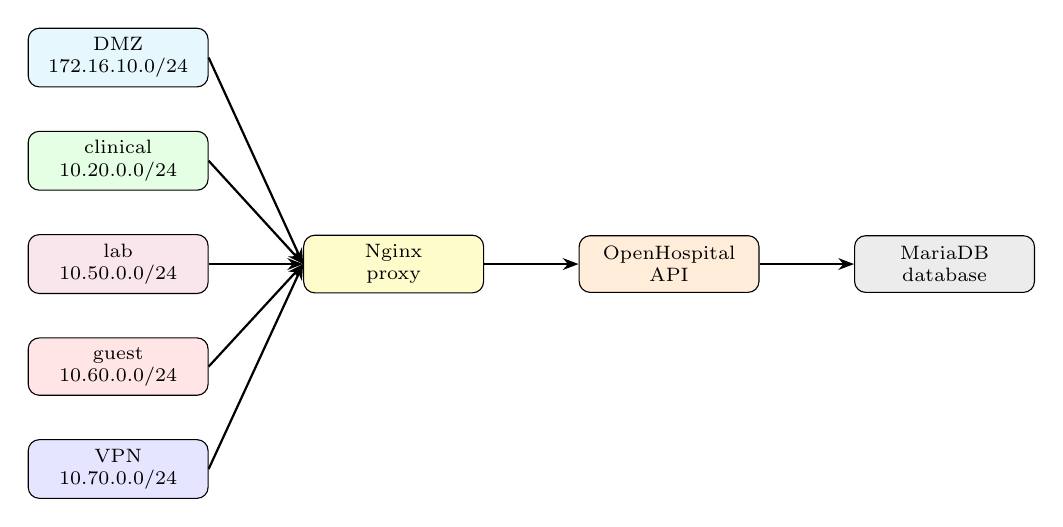
\begin{tikzpicture}[node distance=0.55cm]
\node[labbox, fill=green!10] (clinical) {clinical\\10.20.0.0/24};
\node[labbox, below=of clinical, fill=purple!10] (lab) {lab\\10.50.0.0/24};
\node[labbox, below=of lab, fill=red!10] (guest) {guest\\10.60.0.0/24};
\node[labbox, right=1.2cm of lab, fill=yellow!20] (proxy) {Nginx\\proxy};
\node[labbox, right=1.2cm of proxy, fill=orange!15] (api) {OpenHospital\\API};
\node[labbox, right=1.2cm of api, fill=gray!15] (db) {MariaDB\\database};
\node[labbox, below=of guest, fill=blue!10] (vpn) {VPN\\10.70.0.0/24};
\node[labbox, above=of clinical, fill=cyan!10] (dmz) {DMZ\\172.16.10.0/24};
\draw[labarrow] (dmz.east) -- (proxy.west);
\draw[labarrow] (clinical.east) -- (proxy.west);
\draw[labarrow] (lab.east) -- (proxy.west);
\draw[labarrow] (guest.east) -- (proxy.west);
\draw[labarrow] (vpn.east) -- (proxy.west);
\draw[labarrow] (proxy.east) -- (api.west);
\draw[labarrow] (api.east) -- (db.west);
\end{tikzpicture}
\end{adjustbox}
\end{center}
\end{frame}

\takeawaysframe{
\begin{itemize}
    \item Real deployment adds build, database, and startup dependencies.
    \item Logs are essential during startup.
    \item The proxy should be tested only after the backend is healthy.
\end{itemize}
}{
St. Isidore treats deployment as part of security: an unavailable or misconfigured API cannot be
secured by proxy rules alone.
}

\section{Open Proxy Baseline}
\sectiontitleframe{Open Proxy Baseline}

\begin{frame}[c]{Section Context: Open Proxy Baseline}
\begin{block}{What we are talking about}
The starter Nginx policy forwards every request to OpenHospital API. This is intentionally insecure,
but useful as a baseline.
\end{block}

\begin{exampleblock}{Hospital lens}
At this stage guest Wi-Fi can still reach the API. That is not the final policy; it is the problem
we will fix after proving the deployment works.
\end{exampleblock}
\end{frame}

\begin{frame}[fragile,c]{Starter Proxy Policy}
\begin{block}{Nginx}
\begin{verbatim}
location / {
    proxy_pass http://backend:8080;
}
\end{verbatim}
\end{block}
\end{frame}

\begin{frame}[fragile,c]{Test Healthcheck}
\begin{block}{Commands}
\begin{verbatim}
docker compose exec clinical-client \
  curl -i http://oh-proxy/healthcheck
docker compose exec guest-client \
  curl -i http://oh-proxy/healthcheck
\end{verbatim}
\end{block}

\begin{exampleblock}{Reading the result}
Both should reach the backend in the open baseline. Guest success is evidence that hardening is
still missing.
\end{exampleblock}
\end{frame}

\begin{frame}[fragile,c]{Test Swagger from the DMZ}
\begin{block}{Command}
\begin{verbatim}
docker compose exec dmz-client \
  curl -i http://oh-proxy/swagger-ui/index.html
\end{verbatim}
\end{block}

\begin{exampleblock}{Why Swagger matters}
Swagger confirms that the API is alive and shows endpoint categories such as patients, laboratories,
admissions, users, and authentication.
\end{exampleblock}
\end{frame}

\begin{frame}[c]{Why Swagger Belongs in a DMZ-Like Network}
\begin{block}{Principle}
Swagger and OpenAPI metadata describe the shape of the system. They are useful for operators,
developers, and testers, but they also help an attacker map available operations.
\end{block}

\begin{exampleblock}{Hospital example}
St. Isidore lets a DMZ documentation workstation inspect API contracts. Clinical workstations use
the API they need, but they do not need interactive API documentation during routine care.
\end{exampleblock}
\end{frame}

\begin{frame}[fragile,c]{Test Login}
\begin{block}{Command}
\begin{verbatim}
docker compose exec clinical-client curl -i \
  -H "Content-Type: application/json" \
  -d '{"username":"admin","password":"admin"}' \
  http://oh-proxy/auth/login
\end{verbatim}
\end{block}
\end{frame}

\begin{frame}[c]{Login and Network Control}
\begin{block}{Important distinction}
A successful login proves that application authentication works. It does not prove that the network
exposure is acceptable.
\end{block}

\begin{exampleblock}{Hospital example}
If a guest Wi-Fi device can reach \texttt{/auth/login}, the hospital is letting unmanaged devices
attempt application authentication. The proxy should block that path earlier.
\end{exampleblock}
\end{frame}

\takeawaysframe{
\begin{itemize}
    \item The open proxy baseline proves that the system works.
    \item It also proves that guest reachability exists and must be removed.
    \item Authentication and network exposure are separate layers.
\end{itemize}
}{
St. Isidore uses the open baseline only long enough to confirm that the API, database, and proxy are
functioning.
}

\section{CRUD API Exercise}
\sectiontitleframe{CRUD API Exercise}

\begin{frame}[c]{Section Context: CRUD API Exercise}
\begin{block}{What we are talking about}
Status-code checks prove reachability. CRUD tests prove that the API can perform normal work:
\textbf{create}, \textbf{read}, \textbf{update}, and \textbf{delete} a resource.
\end{block}

\begin{exampleblock}{Hospital lens}
The lab uses \texttt{/admissiontypes}, a small administrative resource, so the exercise changes
disposable training data instead of patient records.
\end{exampleblock}
\end{frame}

\begin{frame}[fragile,c]{Run the CRUD Script}
\begin{block}{Command}
\begin{verbatim}
./crud-admissiontypes.sh
\end{verbatim}
\end{block}

\begin{exampleblock}{What the script does}
It logs in as \texttt{admin}, extracts the JWT token, reads admission types, creates code
\texttt{ZZ}, updates its description, reads again, and deletes it.
\end{exampleblock}
\end{frame}

\begin{frame}[fragile,c]{Call Policy APIs Easily}
\begin{block}{One endpoint}
\begin{verbatim}
./api-call.sh clinical GET /patients?page=0\&size=3
./api-call.sh lab GET /examtypes
OH_NO_AUTH=1 ./api-call.sh dmz GET /swagger-ui/index.html
\end{verbatim}
\end{block}

\begin{exampleblock}{Guided tour}
\texttt{./crud-policy-apis.sh} prints responses for the API paths used in the lab policy, including
allowed calls, denied subnet calls, successful CRUD, and application-level validation errors.
\end{exampleblock}
\end{frame}

\begin{frame}[fragile,c]{CRUD Requests Behind the Script}
\small
\begin{block}{API operations}
\begin{verbatim}
GET    /admissiontypes
POST   /admissiontypes
PUT    /admissiontypes
DELETE /admissiontypes/ZZ
\end{verbatim}
\end{block}

\begin{exampleblock}{Network-security meaning}
These are not just web pages. They are operations that can change hospital configuration data, so
the proxy policy must decide which subnets can reach them.
\end{exampleblock}
\end{frame}

\begin{frame}[fragile,c]{Example Payloads}
\begin{block}{Create and update}
\begin{verbatim}
{"code":"ZZ","description":"SECURITY LAB TRIAGE"}

{"code":"ZZ","description":"SECURITY LAB TRIAGE UPDATED"}
\end{verbatim}
\end{block}
\end{frame}

\takeawaysframe{
\begin{itemize}
    \item CRUD tests confirm useful API behavior, not only reachability.
    \item The JWT proves application authentication is active.
    \item The same endpoint can later be allowed for clinical/VPN and denied for lab/guest.
\end{itemize}
}{
St. Isidore tests a harmless administrative record before applying network restrictions to API
operations.
}

\section{Subnet and Path Policy}
\sectiontitleframe{Subnet and Path Policy}

\begin{frame}[c]{Section Context: Subnet and Path Policy}
\begin{block}{What we are talking about}
The hardened policy combines \textbf{where the request comes from} with \textbf{which API path it
targets}. Nginx access rules can enforce this before OpenHospital API processes the request
\cite{nginx_access}.
\end{block}
\end{frame}

\begin{frame}[fragile,c]{Install the Hardened Policy}
\begin{block}{Commands}
\begin{verbatim}
cp nginx/solution.conf nginx/default.conf
docker compose exec reverse-proxy nginx -s reload
\end{verbatim}
\end{block}
\end{frame}

\begin{frame}[fragile,c]{Guest Network Rule}
\begin{block}{Policy idea}
\begin{verbatim}
deny all;
\end{verbatim}
\end{block}

\begin{exampleblock}{Hospital meaning}
Guest Wi-Fi is for patients and visitors. It should not reach OpenHospital API, Swagger, patient
records, admissions, or laboratory workflows.
\end{exampleblock}
\end{frame}

\begin{frame}[fragile,c]{Laboratory API Rule}
\begin{block}{Policy idea}
\begin{verbatim}
location ^~ /laboratories {
    allow 10.50.0.0/24;
    deny all;
    proxy_pass http://backend:8080;
}
\end{verbatim}
\end{block}
\end{frame}

\begin{frame}[c]{Lab Network Is Not Full Clinical Access}
\begin{block}{Principle}
The laboratory subnet needs laboratory workflows, not unrestricted access to patient administration
or user management endpoints.
\end{block}

\begin{exampleblock}{Hospital example}
The lab may submit or read laboratory results through \texttt{/laboratories}. It should not browse
all \texttt{/patients} endpoints just because it is inside the hospital.
\end{exampleblock}
\end{frame}

\begin{frame}[fragile,c]{Clinical and VPN Rules}
\begin{block}{Policy idea}
\begin{verbatim}
location ^~ /patients {
    allow 10.20.0.0/24;
    allow 10.70.0.0/24;
    deny all;
    proxy_pass http://backend:8080;
}
\end{verbatim}
\end{block}
\end{frame}

\begin{frame}[c]{VPN Is a Controlled Clinical Path}
\begin{block}{Principle}
VPN access should not mean access to every internal system. In this lab, VPN users can reach
clinical API paths through the proxy, but policy can still restrict documentation or administration.
\end{block}
\end{frame}

\begin{frame}[fragile,c]{CRUD Administrative API Rule}
\begin{block}{Policy idea}
\begin{verbatim}
location ^~ /admissiontypes {
    allow 10.20.0.0/24;
    allow 10.70.0.0/24;
    deny all;
    proxy_pass http://backend:8080;
}
\end{verbatim}
\end{block}
\end{frame}

\begin{frame}[c]{CRUD Access Is Still Least Privilege}
\begin{block}{Principle}
An authenticated user is not enough. The request should also arrive from a network where that
operation makes sense.
\end{block}

\begin{exampleblock}{Hospital example}
Clinical administration can maintain admission-type configuration. The laboratory subnet should not
change admission workflow metadata just because lab instruments need lab APIs.
\end{exampleblock}
\end{frame}

\begin{frame}[fragile,c]{DMZ Swagger Rule}
\begin{block}{Policy idea}
\begin{verbatim}
location ^~ /swagger-ui {
    allow 172.16.10.0/24;
    deny all;
    proxy_pass http://backend:8080;
}
\end{verbatim}
\end{block}

\begin{exampleblock}{Hospital meaning}
The DMZ-like documentation network can inspect API contracts. Clinical, lab, guest, and VPN clients
test concrete endpoints instead of browsing the full API map.
\end{exampleblock}
\end{frame}

\takeawaysframe{
\begin{itemize}
    \item Subnet rules answer ``from where?''
    \item Path rules answer ``to which function?''
    \item Least privilege applies to networks, not only users.
\end{itemize}
}{
St. Isidore gives the lab subnet laboratory reachability without turning it into a general clinical
network.
}

\section{Verification}
\sectiontitleframe{Verification}

\begin{frame}[c]{Section Context: Verification}
\begin{block}{What we are talking about}
The hardened policy is only credible if each subnet is tested. A blocked request can be a successful
security result.
\end{block}
\end{frame}

\begin{frame}[fragile,c]{Manual Tests}
\begin{block}{Commands}
\begin{verbatim}
docker compose exec lab-client \
  curl -i http://oh-proxy/laboratories
docker compose exec lab-client \
  curl -i http://oh-proxy/patients
docker compose exec guest-client \
  curl -i http://oh-proxy/healthcheck
docker compose exec dmz-client \
  curl -i http://oh-proxy/swagger-ui/index.html
docker compose exec clinical-client \
  curl -i http://oh-proxy/swagger-ui/index.html
\end{verbatim}
\end{block}
\end{frame}

\begin{frame}[c]{Expected Meaning}
\small
\begin{tabularx}{\textwidth}{@{}p{0.34\textwidth}p{0.18\textwidth}X@{}}
\toprule
\textbf{Request} & \textbf{Expected} & \textbf{Meaning} \\
\midrule
Lab to \texttt{/laboratories} & allowed & lab workflow path works \\
Lab to \texttt{/patients} & \texttt{403} & lab is not full clinical network \\
Guest to \texttt{/healthcheck} & \texttt{403} & guest Wi-Fi is isolated \\
Clinical to \texttt{/patients} & allowed & clinical path works \\
VPN to \texttt{/patients} & allowed & remote clinical path works \\
DMZ to Swagger & allowed & documentation network can inspect API docs \\
Clinical to Swagger & \texttt{403} & care network does not expose API map \\
Clinical to CRUD API & allowed & administrative API path works \\
Lab to CRUD API & \texttt{403} & lab subnet is not administrative \\
\bottomrule
\end{tabularx}
\end{frame}

\begin{frame}[fragile,c]{Automated Check}
\begin{block}{Command}
\begin{verbatim}
./check-policy.sh
\end{verbatim}
\end{block}

\begin{exampleblock}{Reading status codes}
Nginx \texttt{403} means the proxy blocked the request. \texttt{200} or \texttt{401} can both mean
the request reached OpenHospital API, depending on whether the endpoint requires authentication.
\end{exampleblock}
\end{frame}

\begin{frame}[c]{Application Status vs Proxy Status}
\begin{block}{Important}
Network policy testing and application authorization testing are related but not identical.
\end{block}

\begin{exampleblock}{Hospital example}
If the lab subnet receives \texttt{403} for \texttt{/patients}, the proxy blocked it. If it receives
\texttt{401}, the request reached OpenHospital API and the application is asking for authentication.
\end{exampleblock}
\end{frame}

\takeawaysframe{
\begin{itemize}
    \item Test from every relevant subnet.
    \item Interpret status codes by layer.
    \item A good lab result includes command output and explanation.
\end{itemize}
}{
St. Isidore does not trust policy by inspection alone; it proves the behavior from each network.
}

\section{Logs and Investigation}
\sectiontitleframe{Logs and Investigation}

\begin{frame}[c]{Section Context: Logs}
\begin{block}{What we are talking about}
The proxy and OpenHospital API produce different evidence. Both are needed to understand what
happened.
\end{block}
\end{frame}

\begin{frame}[fragile,c]{Read Proxy Logs}
\begin{block}{Command}
\begin{verbatim}
docker compose logs --tail=50 reverse-proxy
\end{verbatim}
\end{block}
\end{frame}

\begin{frame}[fragile,c]{Read Backend Logs}
\begin{block}{Command}
\begin{verbatim}
docker compose logs --tail=100 backend
\end{verbatim}
\end{block}
\end{frame}

\begin{frame}[c]{What Each Log Answers}
\small
\begin{tabularx}{\textwidth}{@{}p{0.25\textwidth}X@{}}
\toprule
\textbf{Log} & \textbf{Question it helps answer} \\
\midrule
Proxy log & Which subnet requested which path, and was it allowed or denied? \\
Backend log & Did the request reach OpenHospital API, and did the API report errors? \\
Application audit & Which authenticated user performed a clinical action? \\
\bottomrule
\end{tabularx}
\end{frame}

\begin{frame}[c]{Design One New Rule}
\begin{block}{Exercise}
Choose one additional policy: allow lab access to \texttt{/patients/search}, deny VPN access to
Swagger, allow guest access only to \texttt{/healthcheck}, or create an admin subnet for
\texttt{/users} and \texttt{/usergroups}.
\end{block}

\begin{exampleblock}{Evidence}
Record the rule, test command, observed status code, and one proxy log line.
\end{exampleblock}
\end{frame}

\takeawaysframe{
\begin{itemize}
    \item Proxy logs show perimeter decisions.
    \item Backend logs show application processing.
    \item New rules should be justified by workflow, not convenience.
\end{itemize}
}{
St. Isidore can explain both blocked guest traffic and allowed clinical API use with evidence.
}

\section{Final Integration}
\sectiontitleframe{Final Integration}

\begin{frame}[c]{Final Concept Map}
\begin{center}
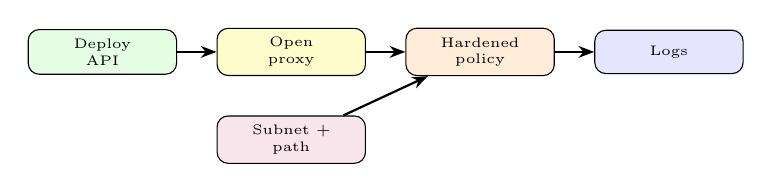
\begin{tikzpicture}[node distance=0.5cm]
\node[smalllabbox, fill=green!10] (deploy) {Deploy\\API};
\node[smalllabbox, right=of deploy, fill=yellow!20] (open) {Open\\proxy};
\node[smalllabbox, right=of open, fill=orange!15] (policy) {Hardened\\policy};
\node[smalllabbox, below=of open, fill=purple!10] (paths) {Subnet +\\path};
\node[smalllabbox, right=of policy, fill=blue!10] (logs) {Logs};
\draw[labarrow] (deploy) -- (open);
\draw[labarrow] (open) -- (policy);
\draw[labarrow] (paths) -- (policy);
\draw[labarrow] (policy) -- (logs);
\end{tikzpicture}
\end{center}

\begin{block}{Reading the map}
Deployment proves the API works. The open proxy proves routing. The hardened policy limits access by
source network and API area. Logs provide evidence for the result.
\end{block}
\end{frame}

\begin{frame}[c]{Final Recap}
\begin{block}{Core lesson}
Network security around a healthcare API is not just ``put it behind Nginx''. The proxy must encode
clinical workflow decisions: guest devices get no access, lab systems get lab APIs, and clinical or
VPN networks get broader but still controlled access.
\end{block}

\begin{exampleblock}{In \scenario}
OpenHospital API remains the application authority, but Nginx reduces who can reach each part of the
API before credentials or tokens are even considered.
\end{exampleblock}
\end{frame}

\begin{frame}[allowframebreaks]{References}
\bibliographystyle{apalike-AMS}
\bibliography{main}
\end{frame}

\end{document}
